%=== Тип документа - статья, кегль 14пт.
\documentclass[14pt]{article}
%=== Настройка кодировок, шрифта и языка
\usepackage[utf8]{inputenc}
\usepackage{textcase}
\usepackage{extsizes}
\usepackage[main=russian, english]{babel}
\usepackage[T2A, T1]{fontenc}

%=== Разметка документа
\usepackage{geometry} 
\geometry{
	a4paper, 
	top = 2cm,
	bottom = 2cm,
	left = 3cm,
	right = 1cm
}
%=== Форматирование текста
\usepackage {setspace}			% Интерлиньяж
\onehalfspacing					% 1.5 строки
\usepackage {indentfirst} 		% Красная строка с первого предложения
\setlength						% Отступ красной строки - 1.25см
	{\parindent}
	{1.25cm}	
\usepackage {titlesec}			% Форматирование заголовков
\titleformat					% Разделы
	{\section}
	[hang]
	{\normalfont\bfseries\centering}
	{\arabic{section}. }
	{0pt}
	{}
\titlespacing
	{\section}
	{\parindent}
	{4ex}
	{0pt}
\titleformat					% Подразделы
	{\subsection}
	[hang]
	{\normalfont\bfseries\itshape}
	{ \arabic{section}.\arabic{subsection}. }
	{0pt}
	{}
\titlespacing
	{\subsection}
	{\parindent}
	{4ex}
	{0pt}
	
\newcommand{\anonsection}[1]{\section*{#1}\addcontentsline{toc}{section}{#1}}
%=== Минимизируем количество переносов
\usepackage {ragged2e}
\usepackage {microtype}
\tolerance = 500
\hyphenpenalty = 20000
\emergencystretch = 1cm
%=== Таблицы
\usepackage {tabularx}	% основной тип таблиц, выравнивание по ширине
\usepackage {longtable}	% для таблиц, не вмещающихся на одну страницу
\usepackage {multirow}	% для разбиения ячеек на несколько строк
\usepackage {multicol}	% на несколько колонок
%=== ^ до этого места - минимальная преамбула документа.
%=== Далее идут опциональные, но часто использущиеся пакеты,
%=== а так же написанные мной команды, чем-то упрощающие написание отчетов

%=== Работа с формулами
% Набор пакетов, сильно расширяющих возможности по набору формул
\usepackage{amsmath}
% добавляет специфические для русских  статей мат. символы вроде \leqslant
\usepackage{amssymb}
% добавляет окружения для теорем и лемм	
\usepackage{amsthm}				
\usepackage{mathtools}
\newcommand{\Mod}[1]{\ (\mathrm{mod}\ #1)}
% номера только для тех формул, на которые есть ссылки в тексте
\mathtoolsset{showonlyrefs=true}
%=== Работа с изображениями
\usepackage{graphicx}
\usepackage{svg}
%=== Работа с гиперссылками
\usepackage[unicode]{hyperref}
\hypersetup{
	colorlinks=true,
	urlcolor=blue,
	filecolor=green,
	linkcolor=red
}

\begin{document}
	\pagenumbering{gobble}
\clearpage
\begin{center}
	\textbf{	
	МИНОБРНАУКИ РОССИИ\\
	САНКТ-ПЕТЕРБУРГСКИЙ ГОСУДАРСТВЕННЫЙ\\
	ЭЛЕКТРОТЕХНИЧЕСКИЙ УНИВЕРСИТЕТ\\
	«ЛЭТИ» ИМ. В.И. УЛЬЯНОВА (ЛЕНИНА)\\
	Кафедра вычислительной техники}

	\vspace{54mm}
	
	\textbf{
	ОТЧЕТ\\
	по учебной практике \\
	Тема: Квантовые вычисления. Алгоритм Шора. \\}

	\vspace{65mm}

	\def\arraystretch{1.5}
	\begin{tabularx}{\textwidth}{ >{\hsize=7cm}X >{\hsize=4cm}X  >{\centering\arraybackslash}X }
		Студент гр. 9308 & & Яловега Н.В. \\ \cline{2-2}
		Руководитель & & Фамилия И.О. \\ \cline{2-2}
	\end{tabularx}
	\def\arraystretch{1}

	\vfill
	Санкт-Петербург\\
	2021
\end{center}
\newpage
\pagenumbering{arabic}
\setcounter{page}{2}
 % титульный лист
	\clearpage

\begin{center}
\textbf{Задание \\ на учебную практику}
 
\end{center}
\begin{flushleft}
Студент Яловега Н.В.

Группа 9308

Тема практики: Квантовые вычисления. Алгоритм Шора.

\vspace{10mm}

Задание на практику:

Изучить основы квантовых вычислений и алгоритмов. Понять принцип работы и реализовать алгоритма Шора.

\vspace{80mm} % удали, когда будешь вставлять текст, это просто для красоты

Сроки прохождения практики: 01.07.2021-14.07.2021

Дата сдачи отчета: 14.07.2021

Дата защиты отчета: 14.07.2021

\end{flushleft}

\begin{center}
	\def\arraystretch{1.5}
	\begin{tabularx}{\textwidth}{ >{\hsize=7cm}X >{\hsize=4cm}X  >{\centering\arraybackslash}X }
		Студент гр. 9308 & & Яловега.Н.В. \\ \cline{2-2}
		Руководитель & & Фамилия И.О. \\ \cline{2-2}
	\end{tabularx}
	\def\arraystretch{1}
\end{center}

\newpage
 % задание
	\clearpage

\begin{center}
\textbf{Аннотация}
\end{center}

	Цель практического задания – добиться понимания принципа работы одного из квантовых алгоритмов и осуществить его реализацию на эмуляторе квантовой системы. В моём случае необходимо проработать квантовый алгоритм факторизации чисел, придуманный в 1994 году Питером Шором.
	
	Для достижения этой цели мне было необходимо усвоить принципы квантовых вычислений, изучить понятия кубита, системы кубитов, и операций над ними. Затем перейти к изучению квантовых алгоритмов и их отличий от классических. Финальным этапом работы стала реализация алгоритма Шора.

%\begin{center}
%\textbf{SUMMARY}
%\end{center}

%Briefly (8-10 lines) to describe the the purpose and main contents of the practice work.


\newpage
 % аннотация
	\tableofcontents 
	
	\newpage
	\anonsection{Введение}
	Кратко описать цель и задачи практики.

	
	\newpage
	\section{Математическая модель квантовых вычислений}
	\subsection{Кубит}
	
	Ключевым понятием всей теории квантовых вычислений является «кубит» — сокращение термина «квантовый бит» (quantum bit) — минимальная информационная единица квантового мира. Так же как бит является частичкой информации, содержащейся в простейшем содержательном классическом вычислительном процессе, кубит является описанием простейшей содержательной квантовой системы.
	
Кубит — это вектор единичной длинны в двумерном гильбертовом пространстве над полем комплексных чисел.
	
	\begin{equation}
	|\phi \rangle \in H, ||\phi|| = 1, dimH = 2;	
	\end{equation}
	
	В гильбертовых пространствах определено скалярное произведение векторов, а значит в можно определить понятие угла $\theta$ между векторами:

	\begin{equation}
	\theta = arccos \frac{ | \langle x|y \rangle | }{||x|| \cdot ||y||}, \theta \in [0, \frac{\pi}{2}];
	\end{equation}

	Выделим в этом пространстве некоторый базис, вектора которого обозначим как $|0 \rangle$ и $|1 \rangle$. Внутри скобок записывается индекс базисного вектора в двоичной системе счисления, начиная с нуля без дополнительных символов.

	\begin{equation}
	|0 \rangle = \begin{bmatrix} 1 \\ 0 \end{bmatrix}, 
	|1 \rangle = \begin{bmatrix} 0 \\ 1 \end{bmatrix};
	\end{equation}

	Тогда произвольный вектор $\phi$ можно выразить следующим образом:
	
	\begin{equation}
	| \phi \rangle = \alpha |0 \rangle + \beta	|1 \rangle,
	\end{equation}
	
	где $\alpha$ и $\beta$ - некоторые комплексные числа, такие что $|\alpha|^2 + |\beta|^2 = 1$
	
	\newpage
	\subsection{Система кубитов}	
	
	В подавляющем большинстве случаев для вычислений требуется более одного бита. Система, состоящая из нескольких кубитов, описывается тензорным произведением составляющих ее систем. Например, квантовый регистр из 2 кубитов будет описываться пространством $H^4$ и иметь 4 базисных состояния.
	
	\begin{equation}
	|00 \rangle = |0 \rangle \otimes |0 \rangle = \begin{bmatrix} 1 \\ 0 \\ 0 \\ 0 \end{bmatrix}
	\end{equation}
	\begin{equation}
	|01 \rangle = |0 \rangle \otimes |1 \rangle = \begin{bmatrix} 0 \\ 1 \\ 0 \\ 0 \end{bmatrix}
	\end{equation}
	\begin{equation}
	|10 \rangle = |1 \rangle \otimes |0 \rangle = \begin{bmatrix} 0 \\ 0 \\ 1 \\ 0 \end{bmatrix}
	\end{equation}
	\begin{equation}
	|11 \rangle = |1 \rangle \otimes |1 \rangle = \begin{bmatrix} 0 \\ 0 \\ 0 \\ 1 \end{bmatrix}
	\end{equation}
	
	Таким образом, система из 3 кубитов описывается вектором в 8-мерном пространстве, а размерность пространства системы из 10 кубитов равна 1024. Для 1000 кубитов мы получаем пространство, размерность которого описывается числом с 300 нулями.
Построив компьютер на всего лишь 1000 атомов, мы получаем в свое распоряжение машину, состояние которой описывается 1030 комплексными числами.
	
	\newpage
	\subsection{Эволюция квантовой системы}
	
	Эволюция квантовой системы унитарна, т.е. любое изменение
ее состояния выражается действием унитарного оператора. Поскольку изменение состояния и есть вычисление, то и программа для квантового компьютера представляет собой последовательное применение различных унитарных операторов к вектору состояния.
Оператор $U$ унитарен, если его сопряженный оператор совпадает с обратным:

	\begin{equation}
	UU^* = U^*U = I
	\end{equation}
	
	Матрица сопряженного оператора представляет собой
транспонированную матрицу исходного оператора, все числа
в которой заменены на сопряженные.
Необходимым и достаточным условием унитарности оператора является сохранение им при отображении длин векторов и углов между ними:

	\begin{equation}
	\forall \phi \in H \text{    } || U|\phi \rangle || = || \phi \rangle ||,
	\end{equation}
	\begin{equation}
	\forall \phi, \psi \in H \text{    } | \langle U|\phi \rangle | U|\psi \rangle \rangle | = | \langle \phi | \psi \rangle |,
	\end{equation}
	
	Несколько примеров наиболее встречающихся операторов:
	
	\textit{Оператор Адамара}:
	\begin{equation}
	H = \frac{1}{\sqrt{2}} \begin{bmatrix} 1 & 1 \\ 1 & -1 \end{bmatrix}
	\end{equation}

	\textit{Гейт X}:
	\begin{equation}
	X = \begin{bmatrix} 0 & 1 \\ 1 & 0 \end{bmatrix}
	\end{equation}	
	
	\textit{Гейт CNOT}:
	\begin{equation}
	X = \begin{bmatrix} 1 & 0 & 0 & 0 \\ 0 & 1 & 0 & 0 \\ 0 & 0 & 0 & 1 \\ 0 & 0 & 1 & 0 \end{bmatrix}
	\end{equation}	

	\newpage
	
	Также для алгоритма Шора нам потребуется квантовый оператор — квантовое преобразование Фурье (Quantum Fourier Transform, QFT):	

	\textit{Квантовое преобразование Фурье}
	\begin{equation}
		N := 2^n
	\end{equation}
	\begin{equation}
		QFT|x \rangle = \frac{||x||}{2^{n/2}} \sum_{y = 0}^{2^n-1}{e^{2 \pi i \frac{xy}{N}}} |y \rangle
	\end{equation}
	
	\newpage
	\subsection{Алгоритм квантовой оценки фазы}
	
	\newpage
	\section{Алгоритм Шора}	
	\subsection{Проблема факторизации}
	Факторизацией натурального числа называется его разложение в произведение простых множителей. Существование и единственность (с точностью до порядка следования множителей) такого разложения следует из основной теоремы арифметики.

В отличие от задачи распознавания простоты числа, факторизация предположительно является вычислительно сложной задачей. В настоящее время неизвестно, существует ли эффективный алгоритм факторизации целых чисел. Даже самым современным алгоритмам требуется экспоненциальное время, чтобы найти коэффициенты целого числа. Это означает, что с достаточно большими числами решить эту задачу практически невозможно, несмотря на огромную вычислительную мощность. Однако доказательства того, что не существует решения этой задачи за полиномиальное время, также нет.

Предположение о том, что для больших чисел задача факторизации является вычислительно сложной, лежит в основе широко используемых алгоритмов (например, RSA).

В 1994 году Питер Шор теоретизировал алгоритм квантовых вычислений с полиномиальным временем для целочисленной факторизации. Алгоритм Шора использует как классические, так и квантовые (определение периода) вычисления. Однако преобладающая оптимизация алгоритма Шора обусловлена эффективностью квантового преобразования Фурье и модульным возведением в степень путем многократного возведения в квадрат.

Алгоритм Шора, используя возможности квантовых компьютеров, способен произвести факторизацию числа не просто за полиномиальное время, а за время, не намного превосходящее время умножения целых чисел (то есть практически так же быстро, как происходит само шифрование).Таким образом, реализация масштабируемого квантового компьютера поставит крест на большей части современной криптографической защиты. Речь не только о схеме RSA, прямо опирающейся на сложности факторизации, но и о других сходных схемах, которые квантовый компьютер способен взломать аналогичным образом.

Важно отметить, что алгоритм Шора имеет вероятностный характер. Первый источник случайности встроен в классическое вероятностное сведение разложения на множители к нахождению периода некоторой функции. Второй источник появляется из необходимости наблюдения квантовой памяти, которое также даёт случайные результаты.
	
	\newpage
	\subsection{Поиск периода и факторизация}
	Алгоритм Шора предназначен для поиска неизвестного периода некоторой периодической функции.
	Как это позволит раскладывать числа на множители?
	
	Пусть $p$ и $q$ - различные простые числа и $N = pq$. Для некоторого числа $a < N: (a, N) = 1$ определим функцию $f_a(x)$:
	
	\begin{equation}
		f_a(x) = a^x \Mod{N}
	\end{equation}
	
	Функция $f_a$ переодическая, и ее период $r$ является порядком числа $a$ в кольце $\mathbb{Z_N}$:
	\begin{equation}
		a^r = 1 \Mod{N}
	\end{equation}
	\begin{equation}
		\forall r_1 < r \text{ } a^{r_1} \neq 1 \Mod{N}
	\end{equation}
	
	Если в нашем распоряжении есть устройство, умеющее находить период любой периодической функции, то при помощи этого устройства, выбрав случайным образом число $a$, мы можем найти период $r$ функции $f_a$.
	
	Допустим, число $r$ - четное. Тогда выражение
	\begin{equation}
		a^r - 1 = 0 \Mod{N}
	\end{equation}
	мы можем представить в виде 
	\begin{equation}
		(a^{r/2} - 1)(a^{r/2} + 1) = Nk
	\end{equation}
	
	Число $(a^{r/2} - 1)$ не делится на $N$, так как иначе $a^{r/2}$ было
бы сравнимо с $0$ по модулю $N$, и число $r/2$ было бы периодом.	
	
	Допустим также, что
	\begin{equation}
		(a^{r/2} + 1) \neq 0 \Mod{N}
	\end{equation}
	
	Тогда произведение $(a^{r/2} - 1)(a^{r/2} + 1)$ делится на $N$, но 
ни один из множителей $(a^{r/2} - 1)$, $(a^{r/2} + 1)$ не делится на $N$
целиком. Следовательно, числа $(a^{r/2} - 1)$, $(a^{r/2} + 1)$ не взаимно
просты с $N$, и мы можем найти $p$ и $q$ при помощи алгоритма Евклида:
	\begin{equation}
		p, q = GCD(a^{r/2} \pm 1, N);
	\end{equation}

	В ходе рассуждения мы сделали два допущения. C какой вероятностью для наугад выбранного числа $a$ его порядок $r$ удовлетворяет этим условиям? Оказывается, что вероятность неудачи сведения задачи факторизации к задаче поиска периода при выборе числа $a$ небольше 1/2
	
	\newpage
	\subsection{Квантовый алгоритм Шора}
	
	Квантовый алгоритм Шора решает проблему нахождения периода следующей функции:
	\begin{equation}
		f(x) = a^x \Mod{N}
	\end{equation}
	
	Решение Шора заключалось в использовании квантовой оценки фазы унитарного оператора:
	\begin{equation}
		U|y \rangle \equiv |ay \text{ } mod \text{ } N \rangle
	\end{equation}
	
	Чтобы увидеть, насколько это полезно, давайте разберемся, как может выглядеть собственное состояние $U$. Если мы начали в состоянии $|1 \rangle$, мы увидим, что каждое последующее применение $U$ будет умножать состояние нашего регистра на $a \Mod{N}$, и после $r$ применений мы снова придем к состоянию $|1 \rangle$. Таким образом, суперпозиция состояний в этом цикле $(|u_0 \rangle)$ будет собственным состоянием $U$:
	\begin{equation}
		|u_0 \rangle = \frac{1}{\sqrt{r}} \sum_{k=0}^{r-1} |a^k \text{ } mod \text{ } N \rangle
	\end{equation}
	
	Это собственное состояние имеет собственное значение 1, что не очень интересно. Более интересным собственным состоянием могло бы быть такое, в котором фаза различна для каждого из этих вычислительных базисных состояний. В частности, давайте рассмотрим случай, когда фаза $k$-го состояния пропорциональна $k$:
	 \begin{equation}
		|u_1 \rangle = \frac{1}{\sqrt{r}} \sum_{k=0}^{r-1} e^{-\frac{2 \pi i k}{r}} |a^k \text{ } mod \text{ } N \rangle
	\end{equation}
	\begin{equation}
		U|u_1 \rangle = e^{\frac{2 \pi i}{r}} |u_1 \rangle
	\end{equation}
	
	Это особенно интересное собственное значение, поскольку оно содержит $r$. Это не единственное собственное состояние с таким поведением; чтобы обобщить это дальше, мы можем умножить целое число $s$ на эту разность фаз, которая будет отображаться в нашем собственном значении: 
	 \begin{equation}
		|u_s \rangle = \frac{1}{\sqrt{r}} \sum_{k=0}^{r-1} e^{-\frac{2 \pi i k s}{r}} |a^k \text{ } mod \text{ } N \rangle
	\end{equation}
	\begin{equation}
		U|u_s \rangle = e^{\frac{2 \pi i s}{r}} |u_s \rangle
	\end{equation}
	
	Теперь у нас есть уникальное собственное состояние для каждого целого значения $0 \le s 
	\le1 r - 1$.
	
	Eсли мы суммируем все эти собственные состояния, разные фазы сокращают все вычислительные базисные состояния, кроме $|1 \rangle$
	\begin{equation}
		 \frac{1}{\sqrt{r}} \sum_{s=0}^{r-1} |u_s \rangle  = |1 \rangle
	\end{equation}
	
	Поскольку вычислительное базисное состояние $|1 \rangle$ является суперпозицией этих собственных состояний, это означает, что если мы выполняем QPE на $U$, используя состояние $|1\rangle$, мы будем измерять фазу:
	\begin{equation}
		 \phi = \frac{s}{r},
	\end{equation}
	где $s$ случайное число между 0 и $r - 1$. Наконец, мы используем алгоритм цепных дробей на $\phi$, чтобы найти $r$. Принципиальная схема выглядит следующим образом:
	\begin{figure}[h!]
		\centering
		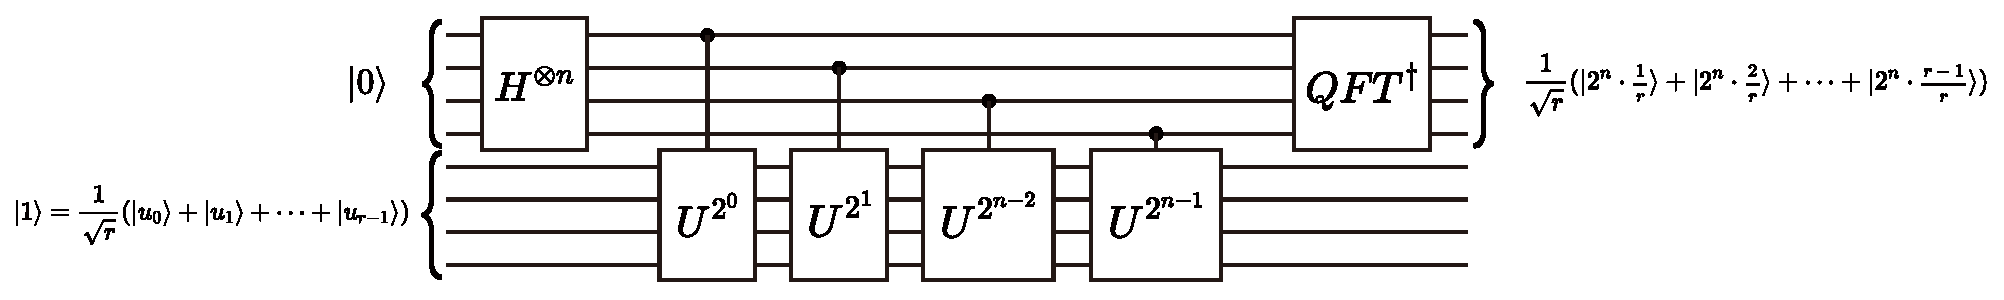
\includegraphics[scale=0.5]{shor_circuit_1}
		\caption{Схема алгоритма Шора}
	\end{figure}

	
	\newpage
	\subsection{Реализация алгоритма}
		
	
	\newpage
	\section{Заключение}
	Кратко подвести итоги, проанализировать соответствие поставленной цели и полученного результата.
	
	\newpage
	\begin{thebibliography}{99}
\addcontentsline{toc}{section}{\bibname}
\bibitem{1}
Сысоев С. С. Введение в квантовые вычисления. Издательство Санкт-Петербургского государственного университета, 2019. 7–109 с.
\bibitem{2}
Курс "Квантовые вычисления (Quantum computing)" [Электронный ресурс] URL: https://www.coursera.org/learn/kvantovyye-vychisleniya
\bibitem{3}
Документация IBM Quantum [Электронный ресурс] URL: https://quantum-computing.ibm.com/lab/docs/
\bibitem{4}
Документация к библиотеке Qiskit [Электронный ресурс] URL: https://qiskit.org/documentation/
\end{thebibliography}

\newpage
	\anonsection{Приложение A}

\begin{center}
\textbf{Исходный код программы}
\end{center}

\newpage


	
\end{document}